\documentclass[fleqn]{article}
\oddsidemargin 0.0in
\textwidth 6.0in
\thispagestyle{empty}
\usepackage{import}
\usepackage{amsmath}
\usepackage{graphicx}
\usepackage{flexisym}
\usepackage{calligra}
\usepackage{amssymb}
\usepackage{bigints} 
\usepackage[english]{babel}
\usepackage[utf8x]{inputenc}
\usepackage{float}
\usepackage[colorinlistoftodos]{todonotes}


\DeclareMathAlphabet{\mathcalligra}{T1}{calligra}{m}{n}
\DeclareFontShape{T1}{calligra}{m}{n}{<->s*[2.2]callig15}{}
\newcommand{\scriptr}{\mathcalligra{r}\,}
\newcommand{\boldscriptr}{\pmb{\mathcalligra{r}}\,}

\definecolor{hwColor}{HTML}{1a0252}

\begin{document}

  \begin{titlepage}

    \newcommand{\HRule}{\rule{\linewidth}{0.5mm}}

    \center

    \begin{center}
      
\includegraphics[height=11cm, width=11cm]{asu.png}
    \end{center}

    \vline

    \textsc{\LARGE Quantum Physics II}\\[1.5cm]

    \HRule \\[0.5cm]
    { \huge \bfseries Problem Set Four}\\[0.4cm] 
    \HRule \\[1.0cm]

    \textbf{Behnam Amiri}

    \bigbreak

    \textbf{Prof: Onur Erten}

    \bigbreak

    \textbf{{\large \today}\\[2cm]}

    \vfill

  \end{titlepage}

  \begin{enumerate}
    \item \textbf{4-10} 
    \begin{enumerate}
      \item Check that $Arj_1(kr)$ satisfies the radial equation with $V(r)=0$ and $\ell=1$.

        \textcolor{hwColor}{
          $
            \\
            \\
            u=A r j_1(kr)
            =A \left[\dfrac{sin(kr)}{r k^2}-\dfrac{cos(kr)}{k}\right]
            =\dfrac{A}{k} \left[\dfrac{sin(kr)}{kr}-cos(kr)\right]
            \\
            \\
            \\
            \dfrac{du}{dr}=\dfrac{A}{k} \left[
              \dfrac{k^2 r cos(kr)-k sin(kr)}{k^2 r^2}
              +k sin(kr)
            \right]
            \\
            \\
            =A \left[\dfrac{cos(kr)}{kr}-\dfrac{sin(kr)}{k^2 r^2}+sin(kr)\right]
            \\
            \\
            \\
            \\
            \dfrac{d^2 u}{dr^2}=A \left[
              -\dfrac{k^2 sin(kr)-k cos(kr)}{k^2 r^2}
              -\dfrac{k^3 r^2 cos(kr)-2k^2 r sin(kr)}{k^4 r^4}
              +k cos(kr)
            \right]
            \\
            \\
            =Ak \left[
              sin(kr) \left(\dfrac{2}{k^3 r^3}-\dfrac{1}{kr}\right)
              cos(kr) \left(1-\dfrac{2}{k^2 r^2}\right)
            \right]
          $
          \\
          \\
          \\
          On page 138 of the textbook we have the radial equation as
          \\
          \\
          \\
          $
            -\dfrac{\hbar^2}{2m} \dfrac{d^2 u}{dr^2}+\left[V+\dfrac{\hbar^2}{2m} \dfrac{\ell (\ell+1)}{r^2}\right]u=Eu
          $
          \\
          \\
          When $V=0$ and $\ell=1$ we have the above equation becomes
          \\
          \\
          $
            \dfrac{d^2 u}{dr^2}-\dfrac{2}{r^2} u=-\dfrac{2 m E}{\hbar^2}u=-k^2 u
            \\
            \\
            \\
            Ak \left[
              sin(kr)\left(\dfrac{2}{k^3 r^3}-\dfrac{1}{kr}\right)
              +cos(kr)\left(1-\dfrac{2}{k^2 r^2}\right)
              -\dfrac{2}{k^2 r^2}\left(\dfrac{sin(kr)}{kr}-cos(kr)\right)
            \right]
            \\
            \\
            \\
            =Ak \left[\dfrac{kr cos(kr)-sin(kr)}{kr}\right]
            \\
            \\
            \\
            =-k^2 u
            \\
            \\
          $
          Hence, we satisfied the radial equation.
          \\
          \\
        }

      \pagebreak

      \item Determine graphically the allowed energies for the infinite spherical well when $\ell=1$.

        \textcolor{hwColor}{
          \\
          On page 140 of the textbook we have $j_{\ell}(ka)=0$. Based on the boundry conditions $j_1(z)=0$ when $z=ka$.
          \\
          \\
          \\
          $
            \therefore ~~~ \begin{cases}
              j_1=\dfrac{sin(z)}{z^2}-\dfrac{cos(z)}{z}=0
              \\
              \\
              z=tan(z)
            \end{cases}
          $
          \\
          \\
          By plotting the two, we can figure out where the intersections are.
          \\
          \\
          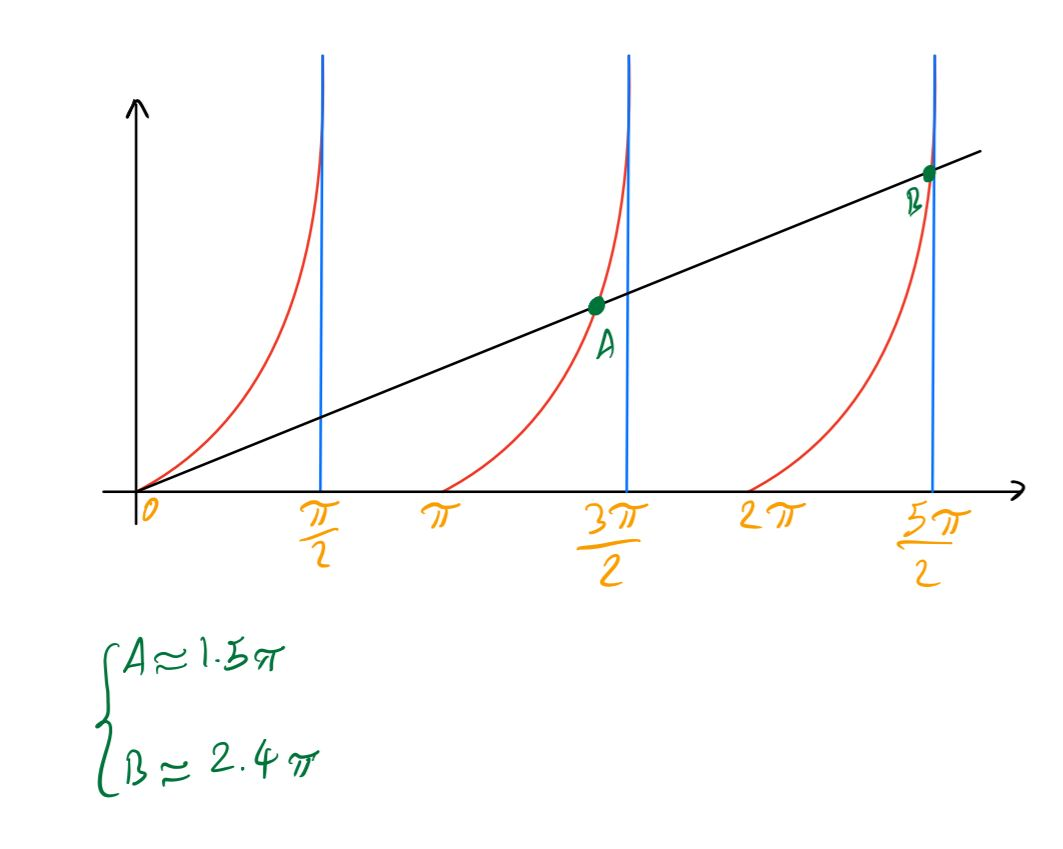
\includegraphics[height=7cm, width=11cm]{Capture.JPG}
          \\
          \\
          \\
          The intersections happen below $z=\pi \left(n+\dfrac{1}{2}\right)$.
          \\
          \\
          \\
          $
            \therefore ~~~ E=\dfrac{\left(\hbar k\right)^2}{2m} \approx \dfrac{\left(\hbar \pi\right)}{2m a^2} \left(n+\dfrac{1}{2}\right)^2
          $
        }

    \end{enumerate}

    \pagebreak

    \item \textbf{4-48} 
    \begin{enumerate}
      \item Prove the three-dimential virial theorem
      $$2\langle T \rangle=\langle r.\nabla V\rangle$$
      (for stationary states). Hint: refer to problem 3.37.

        \textcolor{hwColor}{
          \\
          \\
          Let's recall what the vir­ial the­o­rem is. The vir­ial the­o­rem re­lates the ex­pec­ta­tion ki­netic en­ergy of a quan­tum sys­tem to the po­ten­tial. 
          That is of the­o­ret­i­cal in­ter­est, as well as im­por­tant for com­pu­ta­tional meth­ods like \emph{den­sity func­tional the­ory}.
          Con­sider a quan­tum sys­tem in a state of def­i­nite en­ergy $E$. In other words, con­sider a quan­tum sys­tem in a sta­tion­ary state. 
          \\
          It does not have to be the ground state. The quan­tum sys­tem will be as­sumed to be in in­fi­nite space. To keep it sim­ple, 
          for now as­sume that there is a sin­gle par­ti­cle with po­si­tion vec­tor ${\skew0\vec r}$ in a po­ten­tial $V({\skew0\vec r})$. 
          That cov­ers our pre­vi­ous ex­am­ples of the har­monic os­cil­la­tor and the hy­dro­gen atom.
          Then the vir­ial the­o­rem re­lates the ex­pec­ta­tion ki­netic en­ergy $\left\langle{T}\right\rangle $ to the po­ten­tial $V$ as fol­lows:
          $$2\langle T \rangle=\langle r.\nabla V\rangle$$
          \\
          $
            \dfrac{d}{dt} \langle r.p \rangle=\dfrac{i}{\hbar} \langle \left[H, r.p\right] \rangle
            \\
            \\
            \left[H, r.p\right]
            =\sum\limits_{i=1}^{3} \left[H, r_i p_i\right]
            =\sum\limits_{i=1}^{3} \left(\left[H, p_i\right]r_i+\left[H, r_i\right]p_i\right)
            =\sum\limits_{i=1}^{3} \left(
              r_i \left[V, p_i\right]+p_i \dfrac{1}{2m} \left[p^2, r_i\right]
            \right)
            \\
            \\
            \\
            \left[p^2, r_i\right]
            =\sum\limits_{i=1}^{3} \left[p_j p_j, r_i\right]
            =\sum\limits_{i=1}^{3} \left[p_j \left(-i \delta_{ij}\right)+p_j \left(-i \hbar \delta_{ij}\right)\right]
            \\
            \\
            \\
            \therefore ~~~ \left[p^2, r_i\right]=-2i \hbar p_i ~~~~ \checkmark
          $
          \\
          \\
          Now we need to find $\left[V, p_i\right]$. Recall that
          \\
          \\
          $
            \left[f, p\right]g=f \dfrac{\hbar}{i} \dfrac{dg}{dx}-\dfrac{\hbar}{i} \dfrac{d}{dx} \left(fg\right)
            =f \dfrac{\hbar}{i} \dfrac{dg}{dx}-\dfrac{\hbar}{i} \left(g \dfrac{df}{dx}+f \dfrac{dg}{dx}\right)
            =i g \hbar \dfrac{df}{dx}
            \\
            \\
            \\
            \therefore ~~~ \left[f, p\right]g=i g \hbar \dfrac{df}{dx}
            \\
            \\
            \\
            \therefore ~~~ \begin{cases}
              \left[f, p\right]=i \hbar \dfrac{df}{dx} ~~~~ \checkmark
              \\
              \\
              \left[V, p_i\right]=i \hbar \dfrac{\partial V}{\partial r_i} ~~~~ \checkmark
            \end{cases}
            \\
            \\
            \\
            \left[H, r.p\right]=\sum\limits_{i=1}^{3} \left[
              \dfrac{-i \hbar}{m} p_i p_i +r_i \left(i \hbar \dfrac{\partial V}{\partial r_i}\right)
            \right]
            =i \hbar \left(-\dfrac{p^2}{m}+r. \nabla V\right)
            \\
            \\
            \\
            \dfrac{d}{dt} \langle r.p \rangle
            =\langle \dfrac{p^2}{m}-r. \nabla V \rangle
            =2 \langle T \rangle-\langle r. \nabla V \rangle
          $
          \\
          \\
          Since we are told that our case is for stationary states then $\dfrac{d}{dt} \langle r.p \rangle=0$. Hence,
          \\
          \\
          $
            2 \langle T \rangle-\langle r. \nabla V \rangle=0
            \\
            \\
            \\
            \therefore ~~~ \boxed{
              2 \langle T \rangle=\langle r. \nabla V \rangle ~~~~ \checkmark
            }
          $
          \\
          \\
        }


      \item Apply the virial theorem to the case of hydrogen, and show that
      $$\langle T \rangle=-E_n; ~~~~~ \langle V \rangle=2E_n$$

        \textcolor{hwColor}{
          The hydrogen atom consists of a heavy, essentially motionless proton of charge $e$, with a much lighter electron that orbits around it.
          From Coulomb's law, the potential energy of electron (This is what goes into the Schr$\ddot{o}$dinger equation-not the electric potential
          $e/4 \pi \epsilon_0 r$) is
          $
            V(r)=-\dfrac{e^2}{4 \pi \epsilon_0} \dfrac{1}{r}
            \\
            \\
            \\
            \nabla V=\dfrac{\partial }{\partial r} \left(-\dfrac{e^2}{4 \pi \epsilon_0} \dfrac{1}{r}\right) \hat{r}
            =-\dfrac{e^2}{4 \pi \epsilon_0} \hat{r} \dfrac{d}{dr} \left(\dfrac{1}{r}\right)
            =-\dfrac{e^2}{4 \pi \epsilon_0} \dfrac{-1}{r^2} \hat{r}
            \\
            \\
            \\
            \therefore ~~~ \nabla V=\dfrac{e^2}{4 \pi \epsilon_0} \dfrac{1}{r^2} \hat{r} ~~~~ \checkmark
            \\
            \\
            \\
            r.\nabla V=\left(r \hat{r}\right).\left(\dfrac{e^2}{4 \pi \epsilon_0} \dfrac{1}{r^2} \hat{r}\right)
            =\dfrac{e^2}{4 \pi \epsilon_0} \dfrac{1}{r}
            \\
            \\
            \\
            \therefore ~~~ 2 \langle T \rangle=\langle r. \nabla V \rangle=\langle \dfrac{e^2}{4 \pi \epsilon_0} \dfrac{1}{r} \rangle=-\langle V \rangle
            \\
            \\
          $
          For all atoms and molecules, the motions of the planets $\langle T \rangle=-\dfrac{1}{2} \langle V \rangle$. But for a
          harmonic oscillator, $V=\dfrac{1}{2} kx^2$, $n=2$ so that $\langle T \rangle=\langle V \rangle$ again in either 
          classical or quantum mechanics. Therefore we have the following
          \\
          \\
          $
            \langle T \rangle=\langle V \rangle=E_n \Longrightarrow \langle T \rangle-2\langle T \rangle=E_n
            \\
            \\
            \\
            \therefore ~~~ \boxed{
              \begin{cases}
                \langle T \rangle=-E_n
                \\
                \\
                \langle V \rangle=2 E_n
              \end{cases} ~~~~~~~ \checkmark
            }
            \\
            \\
          $
        }

      \item Apply the virial theorem to the three-dimential harmonic oscillator (problem 4.46), and show that in this case
      $$
        \langle T \rangle=\langle V \rangle=\dfrac{E_n}{2}
      $$

        \textcolor{hwColor}{
          The vir­ial the­o­rem re­lates the ex­pec­ta­tion ki­netic en­ergy of a quan­tum sys­tem to the po­ten­tial.
          \\
          \\
          $
            V=\dfrac{1}{2} ~ m ~ \left(\omega r\right)^2
            \\
            \\
            \nabla V=r ~ m ~ \omega^2 ~ \hat{r} 
            \\
            \\
            \therefore ~~~ \textbf{r}.\nabla V=m ~ \left(\omega ~ r\right)^2
            \\
            \\
          $
          We just showed that $\langle T \rangle=\langle V \rangle$. We know that $\langle T \rangle+\langle V \rangle=E_n$, hence:
          \\
          \\
          $
            \therefore ~~~ \boxed{
              \langle T \rangle=\langle V \rangle=\dfrac{1}{2} E_n
            } ~~~~ \checkmark
          $
        }

      \end{enumerate}

  \end{enumerate}

\end{document}